\documentclass{standalone}
\usepackage{tikz}
\usetikzlibrary{decorations.pathreplacing}
\usepackage{amsfonts}
\usepackage{amsmath}


\begin{document}
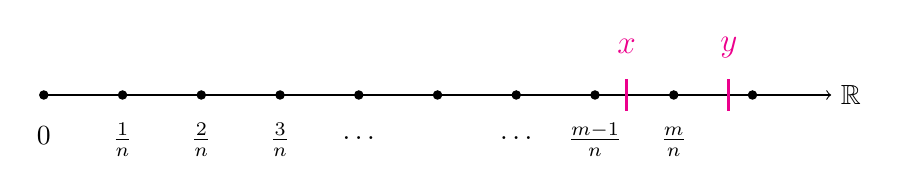
\begin{tikzpicture}
% Draw the real line
  \draw[->] (0,0) -- (10,0) node[right] {$\mathbb{R}$};
  
  % Draw the point 'x' and '0'

 


  \filldraw (0,0) circle (1.5pt);
  \node[anchor=south] at (0,-0.75) {$0$};
  
  \filldraw (1,0) circle (1.5pt);
    \node[anchor=south] at (1,-0.9) {$\frac{1}{n}$};
  
  \filldraw (2,0) circle (1.5pt);
    \node[anchor=south] at (2,-0.9) {$\frac{2}{n}$};

  \filldraw (3,0) circle (1.5pt);
      \node[anchor=south] at (3,-0.9) {$\frac{3}{n}$};
      
  \filldraw (4,0) circle (1.5pt);
        \node[anchor=south] at (4,-0.69) {$\ldots$};
  
  \filldraw (5,0) circle (1.5pt);
  \filldraw (6,0) circle (1.5pt);
          \node[anchor=south] at (6,-0.69) {$\ldots$};
  
  \filldraw (7,0) circle (1.5pt);  
        \node[anchor=south] at (7,-0.9) {$\frac{m-1}{n}$};

  \filldraw (8,0) circle (1.5pt);
        \node[anchor=south] at (8,-0.9) {$\frac{m}{n}$};
  
  \filldraw (9,0) circle (1.5pt);

  
  

  

  

  \draw[line width=1pt, magenta] (7.4,-0.2) -- (7.4,0.2);
  \node[anchor=south, magenta] at (7.4,0.4) {\large$x$};
  
  

  
  \draw[line width=1pt, magenta] (8.7,-0.2) -- (8.7,0.2);
  \node[anchor=south, magenta] at (8.7,0.35) {\large$y$};
  

  
  
  
  \end{tikzpicture}
\end{document}